\documentclass{article}
\usepackage{../FinalYearProjectReport}

% packages for apendicies
\usepackage{color}
\usepackage{listings}
\definecolor{gray}{rgb}{0.4,0.4,0.4}
\definecolor{darkblue}{rgb}{0.0,0.0,0.6}
\definecolor{cyan}{rgb}{0.0,0.6,0.6}

\lstset{
  basicstyle=\ttfamily,
  numbers=left,
  columns=fullflexible,
  showstringspaces=false,
  commentstyle=\color{gray}\upshape
}
\lstdefinelanguage{XML}
{
  morestring=[b]",
  morestring=[s]{>}{<},
  morecomment=[s]{<?}{?>},
  stringstyle=\color{black},
  identifierstyle=\color{darkblue},
  keywordstyle=\color{cyan},
  morekeywords={xmlns,version,type}% list your attributes here
}
\lstdefinelanguage{JavaScript}{
  keywords={typeof, new, true, false, catch, function, return, null, catch, switch, var, if, in, while, do, else, case, break},
  keywordstyle=\color{blue}\bfseries,
  ndkeywords={class, export, boolean, throw, implements, import, this},
  ndkeywordstyle=\color{darkgray}\bfseries,
  identifierstyle=\color{black},
  sensitive=false,
  comment=[l]{//},
  morecomment=[s]{/*}{*/},
  commentstyle=\color{purple}\ttfamily,
  stringstyle=\color{darkblue}\ttfamily,
  morestring=[b]',
  morestring=[b]"
}

% packages for references
\usepackage{cite}
\usepackage{url}


% uncomment this line to double line spacing for proof reading
% \linespread{2}

% packages and settings for graphics
\usepackage{float}
\usepackage[pdftex]{graphicx}
\graphicspath{{./images}}
\DeclareGraphicsExtensions{.png}
\usepackage[final]{pdfpages}


\title{Event Syndication and Dissemination}
\name{Chris Morgan}
\address{Department of Electrical and Computer Engineering\\
University of Auckland, Auckland, New Zealand}


\hyphenation{and-roid}


\begin{document}

\begin{titlepage}


\vspace*{15em}


\centering

{\LARGE Department of Electrical and Computer Engineering\\
Part IV Research Project Report\\
2015}

{\LARGE Event Syndication and Disemination}

\hspace{2em}

% notes on latex tables use "&" as colum sperator
\begin{table*}[h]
\centering
\begin{tabular}{ll}
Project Title: & Event Syndication and Disemination \\
Project Number: & 2 \\
Supervisor Name: & Sathiamoorthy Manoharan \\
Second Examiner Name: & Unknown \\
Your Name: & Chris Morgan \\
Your UID: & 1744263 \\
Partner Name: & Matthew Dyer \\
Date submitted: & \today \\

\end{tabular}
\end{table*}
\begin{table}


\end{table}
\pagebreak

\vspace*{25em}

{\Large Declaration of Originality}

\hspace{5em}

This report is my own unaided work and was not copied from 
nor written in collaboration with any other person.

Name: Chris Morgan 


\end{titlepage}

\maketitle



\begin{abstract}
Think of the abstract as a substitute, for the report, to a busy reader. Its purpose is to enable potential readers to determine whether the contents are likely to be of any interest to them. Thus the abstract must be a summary of the contents of the report, not an overview of the work being reported. To this end it should give abbreviated details of the investigation, why it was commissioned and by whom, its objectives, and its principal results and conclusions.
An abstract should be brief, self-contained and explicit. Although it appears at the beginning of the report, it should be written only after the rest of the report has been completed. It would normally be no longer than 200 words for a major report, and very much less for short reports, such as those described here.
\end{abstract}


\section{Introduction}
The state of conference, convention and summit schedules are scattered. The format they come in is inconsistent, either a pdf, mobile application or website. These schedules are often poorly executed and leave a lot of room for improvement. This project will propose a standard schema for such events and deliver example applications to consume event information compliant with the schema. Conference organisers will be able to use this schema to create schedules that can be viewed and navigated on a diverse range of platforms.

\section{Event Schedules Today}
Event schedules come in a variety of formats; pdfs, mobile applications and websites. Event's like Google IO\cite{googleIO2015}, Embedded Linux Conference\cite{embeddedlinuxconference2015} and Apple WWDC\cite{apple2014wwdc} do it right. They provide an easy platform for attendees to find events, plan their schedules and receive updates. However, there are many events that fall short of providing good schedules. For example, IEEE conference schedules \cite{ieeeIMC2014,ieeePSC2015,ieeeICC2014} leave a lot to be desired.

\section{XML vs. JSON vs. OWL}
Choosing a technology to represent the proposed schema required research into industry standards, trends in web technologies as well as standard library support in a multitude of languages. We looked into three candidates JSON (JavaScript Object Notation), XML (eXtensible Markup Language) and OWL (Web Ontology Language). For the use case of this project, defining a schema in JSON or XML is equivalent apart from syntax. Neither technology offers significant advantages or disadvantages. OWL on the other hand, while it has some innovative advantages is, not on par with the others.

\subsection{XML}
When we started this project, XML was the technology that our supervisor recommended we use. It's understandable that it should be the obvious choice, as it is the most widely used resource type in APIs\cite{maleshkova2010investigating}. XML is mature language, first released in 1996 and is used extensively by Microsoft and integrates well into .Net and Java applications. XSD (XML Schema Definition) is the language used to describe XML schemas and is what would have been used if XML was chosen. The XSD, like most schema definition languages enables the creation of data types, inheritance and validation of data. One of the main inspirations of this project, RSS (Rich Site Summary or Really Simple Syndication) is defined using XSD along with many other XML based data transfer specifications.

\subsection{JSON}
Over the last few years, use of JSON in transferring over the internet and storing data as been increasing in popularity as seen in figure~\ref{fig:JSON_XML_all_time}. This is in part due to the increase in the usage of front end web application frameworks such as React, AngularJS, Ember.js and Backbone.js. It's no surprise that JSON is easier, faster and cleaner \cite{hellstrom2012querying,lin2012comparison,nurseitov2009comparison} to work with using it's namesake, JavaScript rather than XML. As one of the primary outcomes of this project is to create an example web application, this ease of use plays heavily when choosing which technology to use.
\begin{figure}[h]
	\centering
	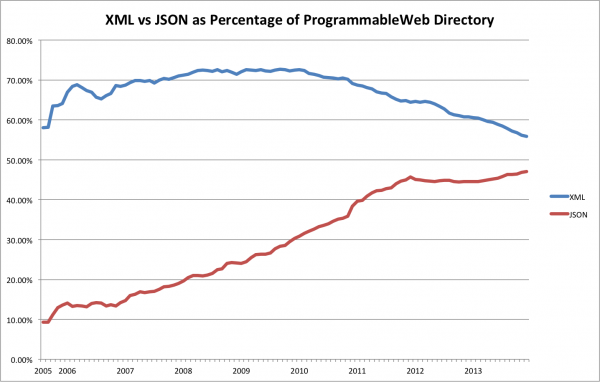
\includegraphics[scale=0.37]{images/xml_json_all_time.png}
	\caption{Overall XML vs. JSON Use\protect\cite{duvander2013json}}
	\label{fig:JSON_XML_all_time}
\end{figure}

\subsection{OWL}

\section{Defining a schema}
The first stage of the project was developing a schema to encapsulate conference information. We looked at a multitude of conference schedules as well as mobile applications to understand the scope of what our schema would need to contain. See listing~\ref{lst:jsonSchema} on page~\pageref{lst:jsonSchema} for the preliminary schema definition. The proposed schema has room for improvement but contains the basic information needed to navigate a conference. Matthew focused more on what should be in the schema while I focused on the technology behind the schema.

\section{Evaluation}

\section{Future project plan}

\section{Conclusion}
The conclusions are intended to emphasise what the author considers to be the significant findings or outcome of the investigation. They are a restatement of the essential information that the author has tried to impart to the reader. The primary value of a report derives from the nature, originality and soundness of the conclusions. They must be presented clearly and succinctly.

\bibliographystyle{IEEEtran}
\bibliography{cmor149}

\onecolumn
\appendix
\section{Schemas}
% \lstinputlisting[caption=XML Schema Description, language=XML]{../schema/esad.xsd}
\lstinputlisting[caption=JSON Schema Description, language=JavaScript, label={lst:jsonSchema}]{../../schema/esad.schema.json}


\end{document}